\chapter{Review}

As seen in the last chapter, the implemented document scanner successfully scanned all of the test images provided. Summarized, an exemplary step-by-step overview of the scanning process can be seen in \autoref{fig:overall}.

Of course, only further usage will tell whether the found algorithm works for a wide variety of documents, table surfaces, lighting conditions, camera qualities and more. For this, a bigger amount of test images would be needed, alongside the necessary adjustments to thresholds or values in the algorithm. With todays machine learning algorithms, this could possibly be done even without human work.

\begin{figure}[h]
    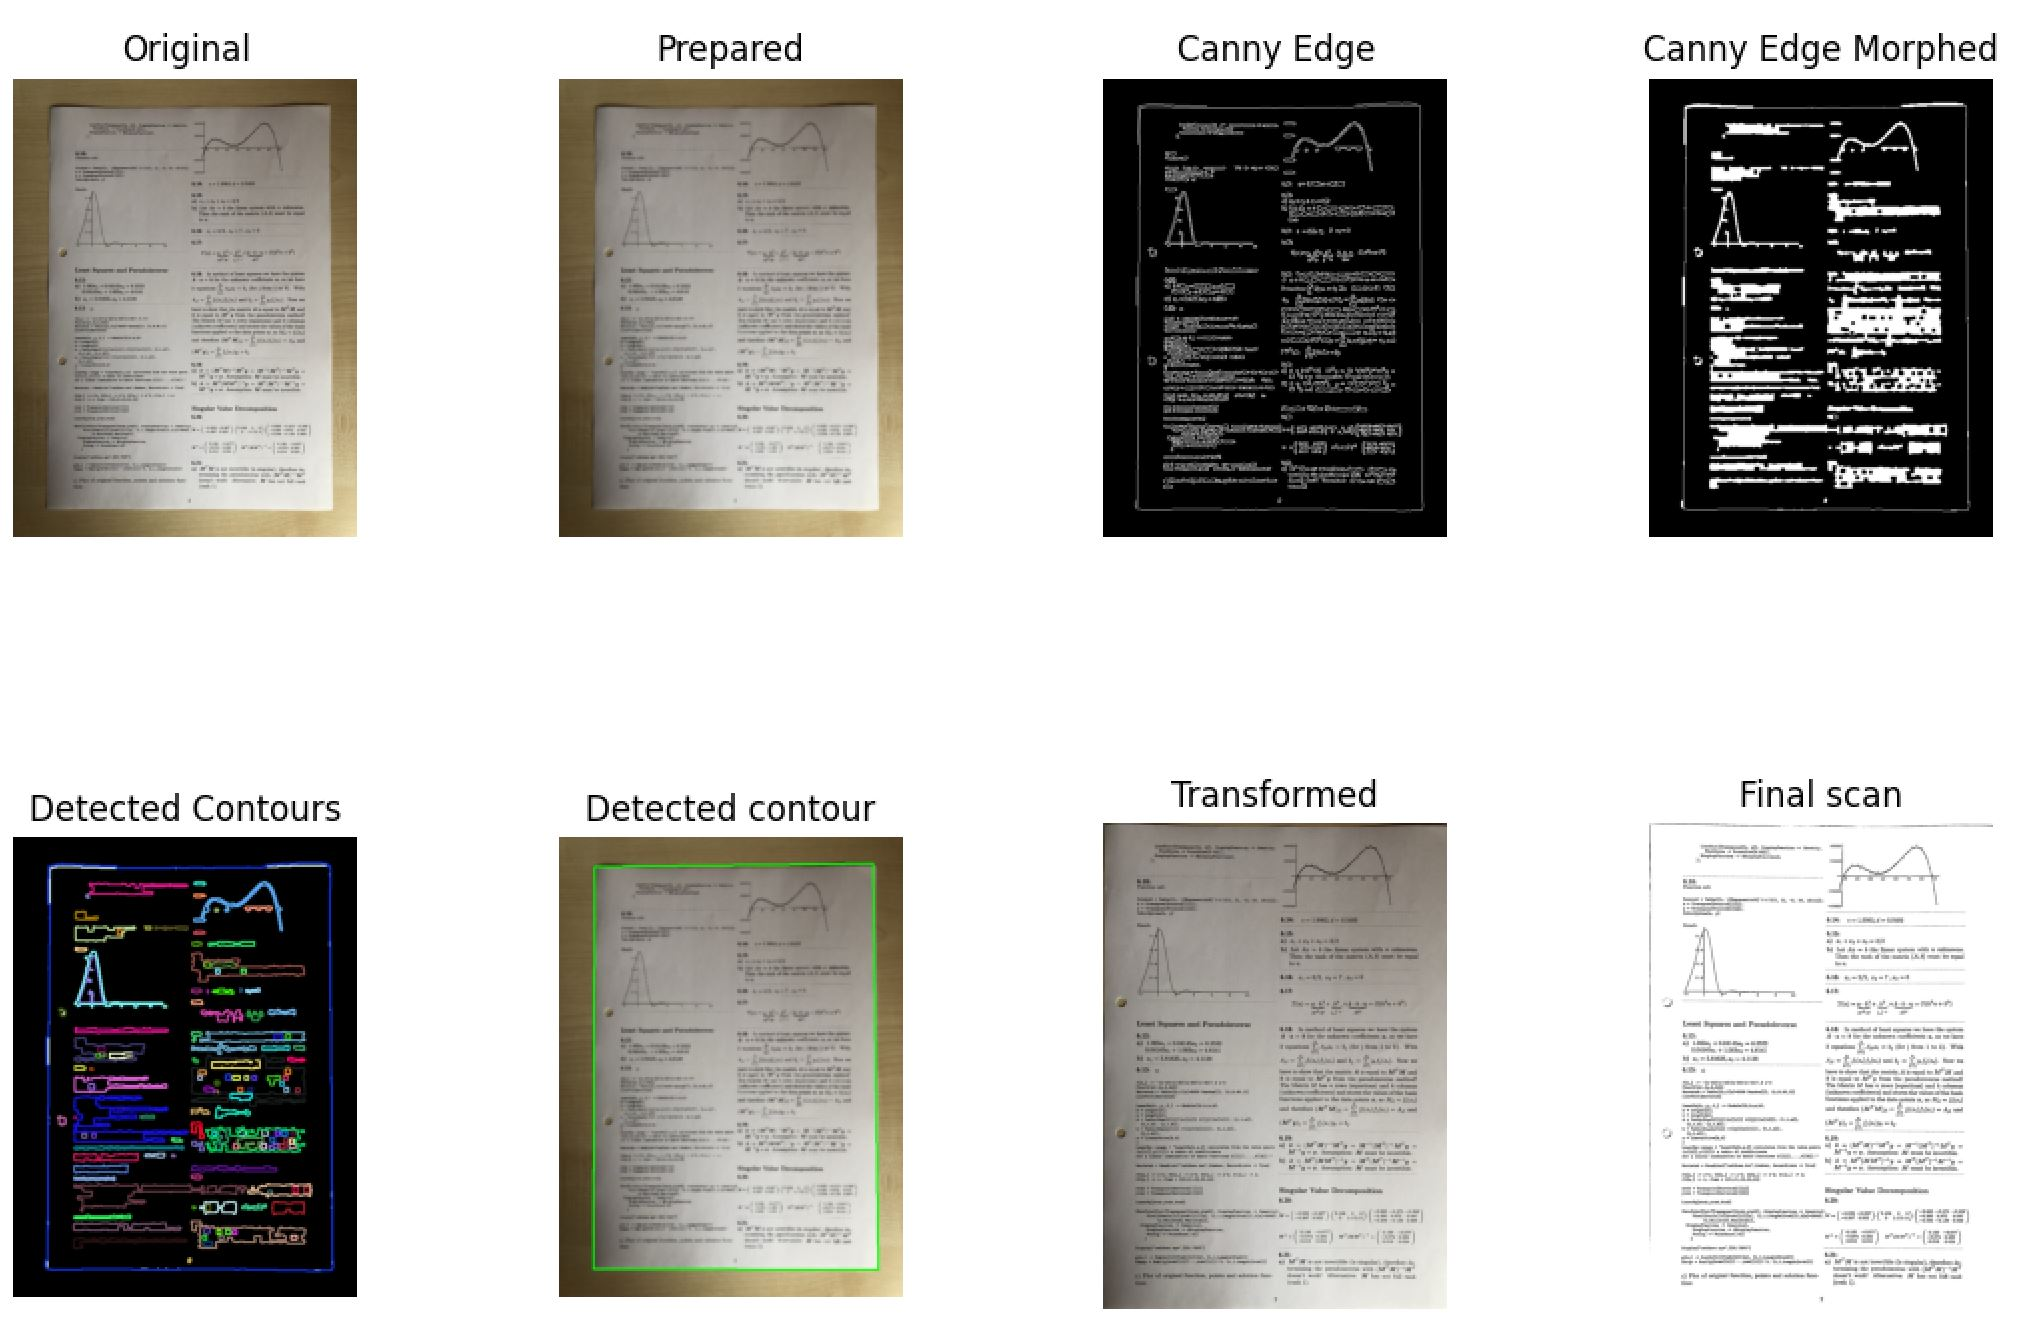
\includegraphics[width=1\textwidth]{figures/allsteps.jpg}
    \centering
    \caption{Step-by-step scan of a document}
    \label{fig:overall}
\end{figure}

Although not part of the exercise, the scanner was also tested with colored documents and non-standard-sized documents. The scanner returned mixed results there.

The scan of a colored advertisement sheet, having a non-standard size, worked without further changes, as can be seen in \autoref{fig:colored}. The particular advertisement sheet had the difficulty of additional square boxes inside the document that could have been detected as the document contours.

\begin{figure}[h]
    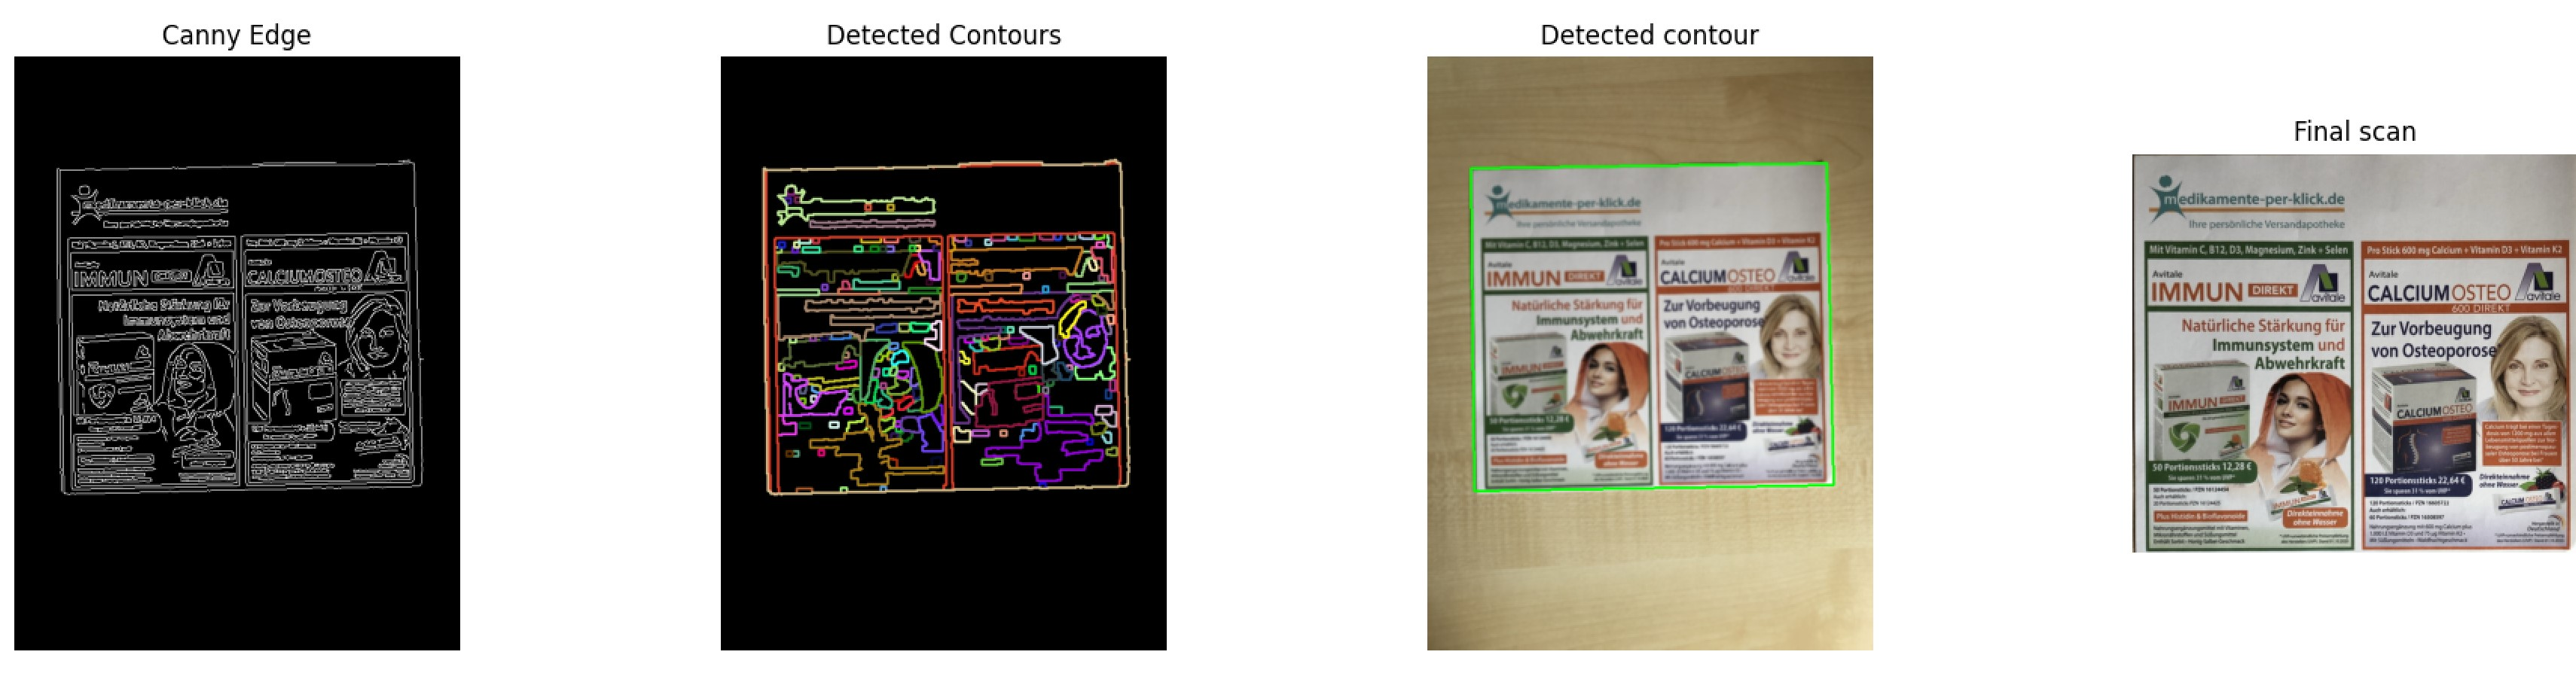
\includegraphics[width=1\textwidth]{figures/colored.jpg}
    \centering
    \caption{Successful scan of colored non-standard sheet}
    \label{fig:colored}
\end{figure}

On the other hand, scanning of a colored magazine cover didn't work, as seen in \autoref{fig:konzepte}. While the edge of the purple part of the cover was detected, the lower white-grey part of the cover was not detected, resulting in an incomplete outer shape that couldn't be recognized as a square. Possibly the detection could be fixed by altering the thresholds, but this would at the same time change the detection rate of other documents.

\begin{figure}[h]
    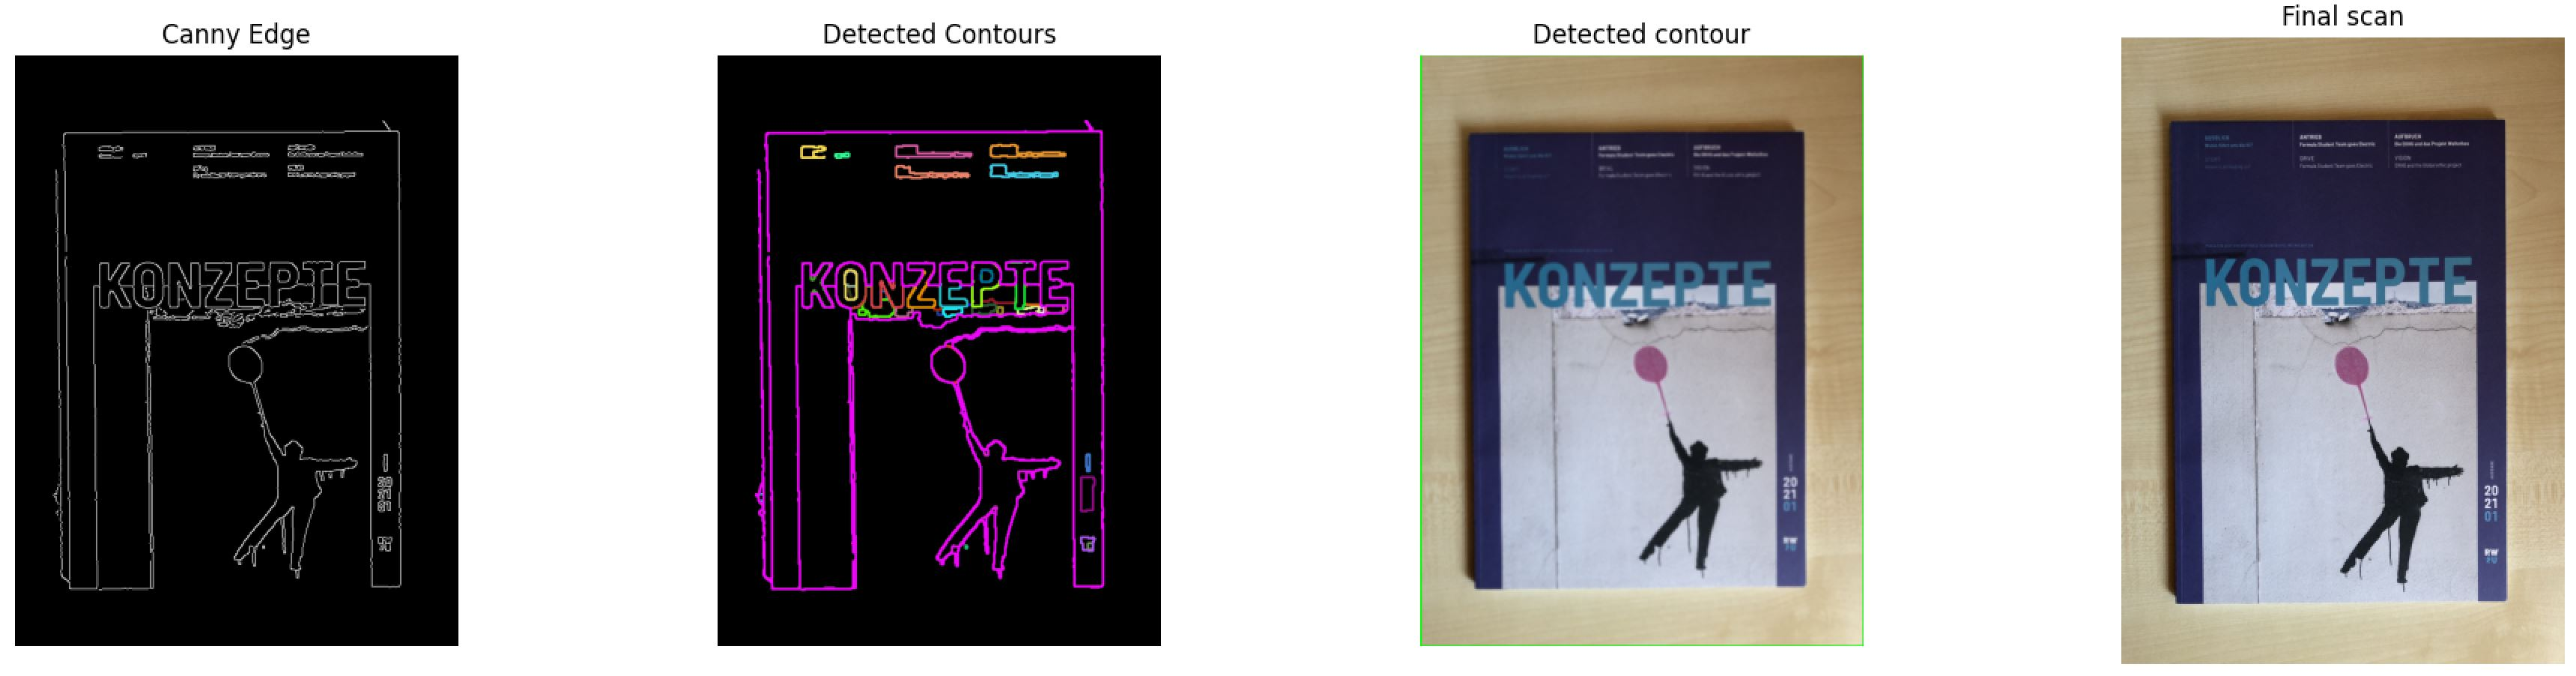
\includegraphics[width=1\textwidth]{figures/konzepte.jpg}
    \centering
    \caption{Unsuccessful scan of colored magazine}
    \label{fig:konzepte}
\end{figure}